\documentclass[assignment03_Solutions]{subfiles}

\IfSubStr{\jobname}{\detokenize{Solutions}}{\toggletrue{solutions}}{\toggletrue{solutions}}

%\IfSubStr{\jobname}{\detokenize{Solutions}}{\toggletrue{solutions}}{\togglefalse{solutions}}

\fancypagestyle{firstpage}

{\rhead{Assignment 1 \linebreak \textit{Version: \today}}}

\title{Assignment 3: Classification, Logistic Regression, and Gradient Descent}
\author{Machine Learning}
\date{Fall 2019}

\begin{document}

\maketitle
\thispagestyle{firstpage}


\begin{learningobjectives}
\bi
\item Learn about the framing of the classification problem in machine learning.
\item Learn about the logistic regression algorithm.
\item Learn about gradient descent for optimization.
\item Some C\&E topic.
\ei
\end{learningobjectives}

\begin{priorknowledge}
\bi
\item Supervised learning problem framing.
\item Training / testing splits.
\ei
\end{priorknowledge}
\vspace{1em}


\begin{recall}[Supervised Learning Problem Setup]
We are given a training set, $(\mlvec{x_1}, y_1), (\mlvec{x}_2, y_2), \ldots, (\mlvec{x}_n, y_n)$ where each $\mlvec{x_i}$ represents an element of an input space (e.g., a d-dimensional feature vector) and each $y_i$ represents an element of an output space (e.g., a scalar target value).  Our goal is to determine a function $\hat{f}$ that maps from the input space to the output space.

We assume there is a loss function, $\ell$, that determines the amount of loss that a particular prediction $\hat{y}_i$ incurs due to a mismatch with the actual output $y_i$.  The best possible model, $\hat{f}^\star$, is the one that minimizes these losses over the training set.  This notion can be expressed with the following equation.
\begin{align}
\hat{f}^\star &= \argmin_{\hat{f}} \sum_{i=1}^n \ell \left ( \hat{f}(\mlvec{x_i}), y_i \right )
\end{align} 
\end{recall}


\section{The Classification Problem}

So far in this class we've looked at supervised learning problems where the responses $y_i$ are continuous-valued and the loss function is quadratic ($\ell(y, \hat{y}) = (y-\hat{y})^2$).  This is an example of a regression problem.  There are many times, however, where it is unnatural to frame a problem as a regression.  For instance, it may be the case that $y_i$ does not come from a continuous range but can only take on a few different values.  This sort of problem is known as a classification problem.  For instance, you might want to have a system that can take in an image of a person and predict their identity.  The identity could be thought of as the output, $y_i$, and it could only take on one of several values (each value might represent a particular person the system was trained to recognize).  In this assignment you'll learn about a special case of the classification problem known as binary classification (where $y_i$ is either 0 or 1, e.g., a Paul versus Sam detector).

In this assignment will formalize the binary classification problem and see a very useful algorithm for solving it called \emph{logistic regression}.  You will also see that the logistic regression algorithm is a very natural extension of linear regression.  Our plan for getting there is going to be pretty similar to what we did for linear regression.
\bi
\item Build some mathematical foundations
\item Introduce logistic regression from a top-down perspective
\item Learn about logistic regression from a bottom-up perspective
\ei

\section{Formalizing the Classification Problem}
Let's start by making the binary classification problem more formal.  Suppose, we are given a training set, $(\mlvec{x_1}, y_1), (\mlvec{x}_2, y_2), \ldots, (\mlvec{x}_n, y_n)$, where each $\mlvec{x_i}$ is an element of the input space (e.g., a vector) and each $y_i$ is a binary number (either 1 or 0).  In this setting we will attempt to use the training data to determine a function, $\hat{f}^\star$, that predicts the corresponding output, $y$, for any possible input, $\mathbf{x}$.  To make this concrete with an example,  $\mathbf{x}$ could be an image and $y$ could be a binary number that takes on value $1$ when the picture contains a puppy.


\begin{exercise}[(10 minutes)]
\bes
\item Given this setup of the binary classification problem, the only thing left to specify is the loss function, $\ell$.  Recall that $\ell$ takes as input the actual output $y$, and the predicted output $\hat{y}$.  What function could you use for $\ell$ that would result in the learning algorithm choosing a good model.  If the choice of $\ell$ depends on the application, how so?

\begin{boxedsolution}
An easy choice is to output a $1$ if the values don't match and a $0$ otherwise (essentially counting the number of mistakes the model makes).  Alternatively, you could have different penalties for a false positive (the model says $\hat{y} = 1$, but the actual value is $y = 0$) or false negatives (the model says $\hat{y} = 0$, but the actual value is $y = 1$). 
\end{boxedsolution}

\item \label{ex:minmistakes}
One natural choice, that you may have already come up with in the previous question, is to define our loss function as $\ell(y, \hat{y}) = \mathbb{I}[y \neq \hat{y}]$ (the funny looking $\mathbb{I}$ is the indicator function that takes on value 1 when the condition inside is true and 0 otherwise.  Given these choices, the supervised learning problem becomes:
\begin{align}
\hat{f}^\star &= \argmin_{\hat{f}} \sum_{i=1}^n \mathbb{I} \left [  \hat{f}(\mlvec{x_i}) \neq, y_i\right ] \enspace . \label{eq:minimizeerror}
\end{align}

Convert Equation~\ref{eq:minimizeerror} to English to make sure you understand it.
\begin{boxedsolution}
The equation says that $\hat{f}^\star$ is the function $\hat{f}^\star$ that minimizes the number of mistakes that the function makes on the training set.
\end{boxedsolution}

\ees

\end{exercise}

The loss function given in Exercise~2\ref{ex:minmistakes} is a totally reasonable choice since it will result in choosing the model that makes the fewest mistakes on the training.  It turns out, however, that it has the following drawbacks.
\bi
\item It is all or nothing.  Either we are completely right or completely wrong.
\item It is not a particularly easy function to work with mathematically.  In fact, for many common classes of models, it will be difficult for the learning algorithm to find the best possible model\sidenote{One of the key challenges that must be in met in machine learning, and modeling in general, is balancing computational considerations (e.g., how long does it take to find the best possible model) with the realism of the model (e.g., how directly does the task you pose to the learning algorithm match the problem you are solving.  Sometimes these things are in conflict and you must make tradeoffs.}.
\ei
It turns out that we can create a much more natural loss function by thinking about predictions in terms of probabilities.

\section{Probability and the log loss}
Imagine that instead of our model, $\hat{f}$, spitting out either 0 or 1, it outputs a confidence that the input $x_i$ has an output, $y_i$, that was 1.  In other words, rather than giving us its best guess, the classifier would indicate to us its degree of certainty regarding its prediction.  This notion of ``certainty'' can be formalized using the concept of a probability.  That is, the model can output a probability that the output for a particular input is 1.

We haven't formally defined probability in this class, and we won't do so here (we'll be working with probabilities extensively in module 2 and we don't need a formal treatment to derive the classification algorithms we will study in this module).  Here are a few things to keep a few things in mind about probabilities.
\bi
\item A probability, $p$, specifies the chance that some event occurs ($p = 0$ means that the even will definitely not occur and $p=1$ means that it will definitely occur.
\item A probability, $p$, must be between 0 and 1 ($0 \leq p \leq 1$).
\item If the probability an event occurs is $p$, then the probability that the event doesn't occur is $1 - p$.
\ei

\begin{understandingcheck}
\textbf{Note: these sorts of boxes are here to help you test your understanding of a concept you have just read.  We are trying to use these to breakup long blocks of reading.  You do not need to submit these.}

TODO: Quick check of understanding
\end{understandingcheck}

\subsection{Log loss}
Thinking back to the binary classification problem, if we think in terms of probability, then our model output a probability $p$ when supplied with an input $\mlvec{x}$ (i.e., $\hat{f}(\mlvec{x}) = p$).  We might then ask ourselves the question of what would be a reasonable loss function to quantify how good a prediction $p$ is given the actual output $y$ (recall that for the binary classification the output is either $0$ or $1$).  To make to this more intuitive, consider the task of quantifying the quality of a weatherperson's predictions.  Further, let's assume that on any given day the weather is either sunny (call this output $1$) or rainy (call this output $0$).  Suppose that each night the weather person provides a probability that indicates the chance of it being sunny the next day.  In order to quantify the loss of each prediction we need to define a loss function.  Here are two potential choices.
\be
\item \textbf{0-1 loss:} we will extract from the weatherperson's prediction the most likely outcome (e.g., if $p = 0.75$, that would be sunny, if $p = 0.4$, that would be rainy).  If this most likely outcome matches the actual outcome we give a loss of 0, otherwise we give a loss of 1 (this is similar to Equation~\ref{eq:minimizeerror}).
\item \textbf{squared loss:} one downside of \emph{0-1 loss} is that it doesn't take into account the certainty expressed by the weatherperson.  The weatherperson gets the same loss if it is rainy and they predicted $p = 0.51$ or $p = 1$.  For squared loss we can compute the difference between the outcome and $p$ and square it to arrive at the loss.  So if we predict $p = 0.51$ and it is sunny we get a loss of $(1 - 0.51)^2$.  If it was rainy in this same example, we get a loss of $(0 - 0.51)^2$.
\ee

As an example, here are hypothetical predictions from two forecasters, the actual weather, and the resulting loss with either \emph{0-1} loss or \emph{squared loss}.


\begin{table*}
\centering
\small
\begin{tabular}{c | c | c | c | c | c | c}
\hline
actual weather & forecast 1 & 0-1 loss & squared loss & forecast 2 1 & 0-1 loss & squared loss \\
\hline
\mbox{sunny (y = 1)} & $p = 0.3$ & 1 & $(1-0.2)^2 = 0.64$ & $p = 0.9$ & 0 & $(1 - 0.9)^2 = 0.01$\\
\mbox{rainy (y = 0)} & $p = 0.6$  & 1 & $(0-0.6)^2 = 0.36$ & $p = 0.999$ & 1 & $(0 - 0.999)^2 = 0.998$ \\ 
\mbox{sunny (y = 1)} & $p = 0.8$ & 0 & $(1-0.8)^2 = 0.16$ & $p = 0.99$ & 0 & $(1 - 0.99)^2 = 0.0001$\\
\hline
\textbf{average} & & $0.667$ & $0.347$ & & 0.333 & 0.336
\end{tabular}
\end{table*}

\normalsize % I don't think we actually need this.

\begin{understandingcheck}
According to the table above, which forecaster is better with regards to \emph{0-1 loss}?  Which forecaster is better with regards to \emph{squared loss}?
\end{understandingcheck}

One entry in the table above is particularly interesting.  In the third row, the second forecaster assigned a probability of $0.999$ to the fact that it was going to be sunny.  It turned out to rain (boo!!!).  That is, the forecaster was almost certain it would be sunny and it wasn't.  The 0-1 loss of course doesn't capture this at all.  The squared loss seems to assign a fairly large loss.  One might argue, though, that this loss does not fully capture how bad the prediction was.  This last observation motivates a third loss function that we can use to evaluate probabilistic predictions: the log loss.

\begin{externalresources}
\url{wiki.fast.ai} has some really nice resources on a number of topics.  They have a nice concise writeup that explains the concept of log loss.  We ask that you read about \href{http://nb.mit.edu/f/55213}{log loss on NB} so you can take advantage of some notes from us to help guide your reading and add your own notes as well.  If you want the original page (e.g., to click on the links), you can access the \href{http://wiki.fast.ai/index.php/Log_Loss}{log loss page on wiki.fast.ai}.
\begin{exercise}
TODO Here are some questions to test your understanding of the log loss reading.
\end{exercise}
\end{externalresources}

\section{Logistic Regression (top-down)}
Now that we have built up some understanding of how probabilities can be used as a way of quantifying confidence in predictions, you are ready to learn about the logistic regression algorithm.

As always, we assume we are given a training set of inputs and outputs.  As in linear regression we will assume that each of our inputs is a $d$-dimensional vector $\mathbf{x_i}$ and since we are dealing with binary classification, the outputs, $y_i$, will each be binary numbers (indicating whether the corresponding input is of class 0 or 1).  Our hypothesis functions, $\hat{f}$, output the probability that a given input has a corresponding output of 1.  Each $\hat{f}$ has the following form (note: this equation will look daunting, so we have some tips for interpreting it below).

\begin{align}
\hat{f}(\mathbf{x}) &= \mbox{probability that $y$ is 1 for $\mlvec{x}$} \nonumber \\
&=\frac{1}{1 + e^{-\mlvec{w}^\top \mathbf{x}}}
\end{align}

Here are a few things to notice about this equation:
\be
\item The weight vector that we saw in linear regression, $\mlvec{w}$, is making a comeback!  In fact, we have a dot product between $\mlvec{x}$ and $\mlvec{w}$ (which creates a weighted sum of the $x_i$'s) just as we did in linear regression.
\item Despite the similarities with linear regression, we now have this super weird term involving $\frac{1}{1+e^{-\mbox{stuff}}}$.  It turns out that this function is known as the logistic function, $\sigma$.  The graph of $\sigma(u) = \frac{1}{1+e^{-u}}$ is shown in Figure~\ref{fig:sigmoid}.  The function acts to map any real number to a number between 0 and 1.  Thus it is a perfect ``squashing'' function to take numbers that might not necessarily be valid probabilities (e.g., $\mlvec{w}^\top \mlvec{x}$) and squash them to the range of valid probabilities $[0,1]$.

\begin{marginfigure}
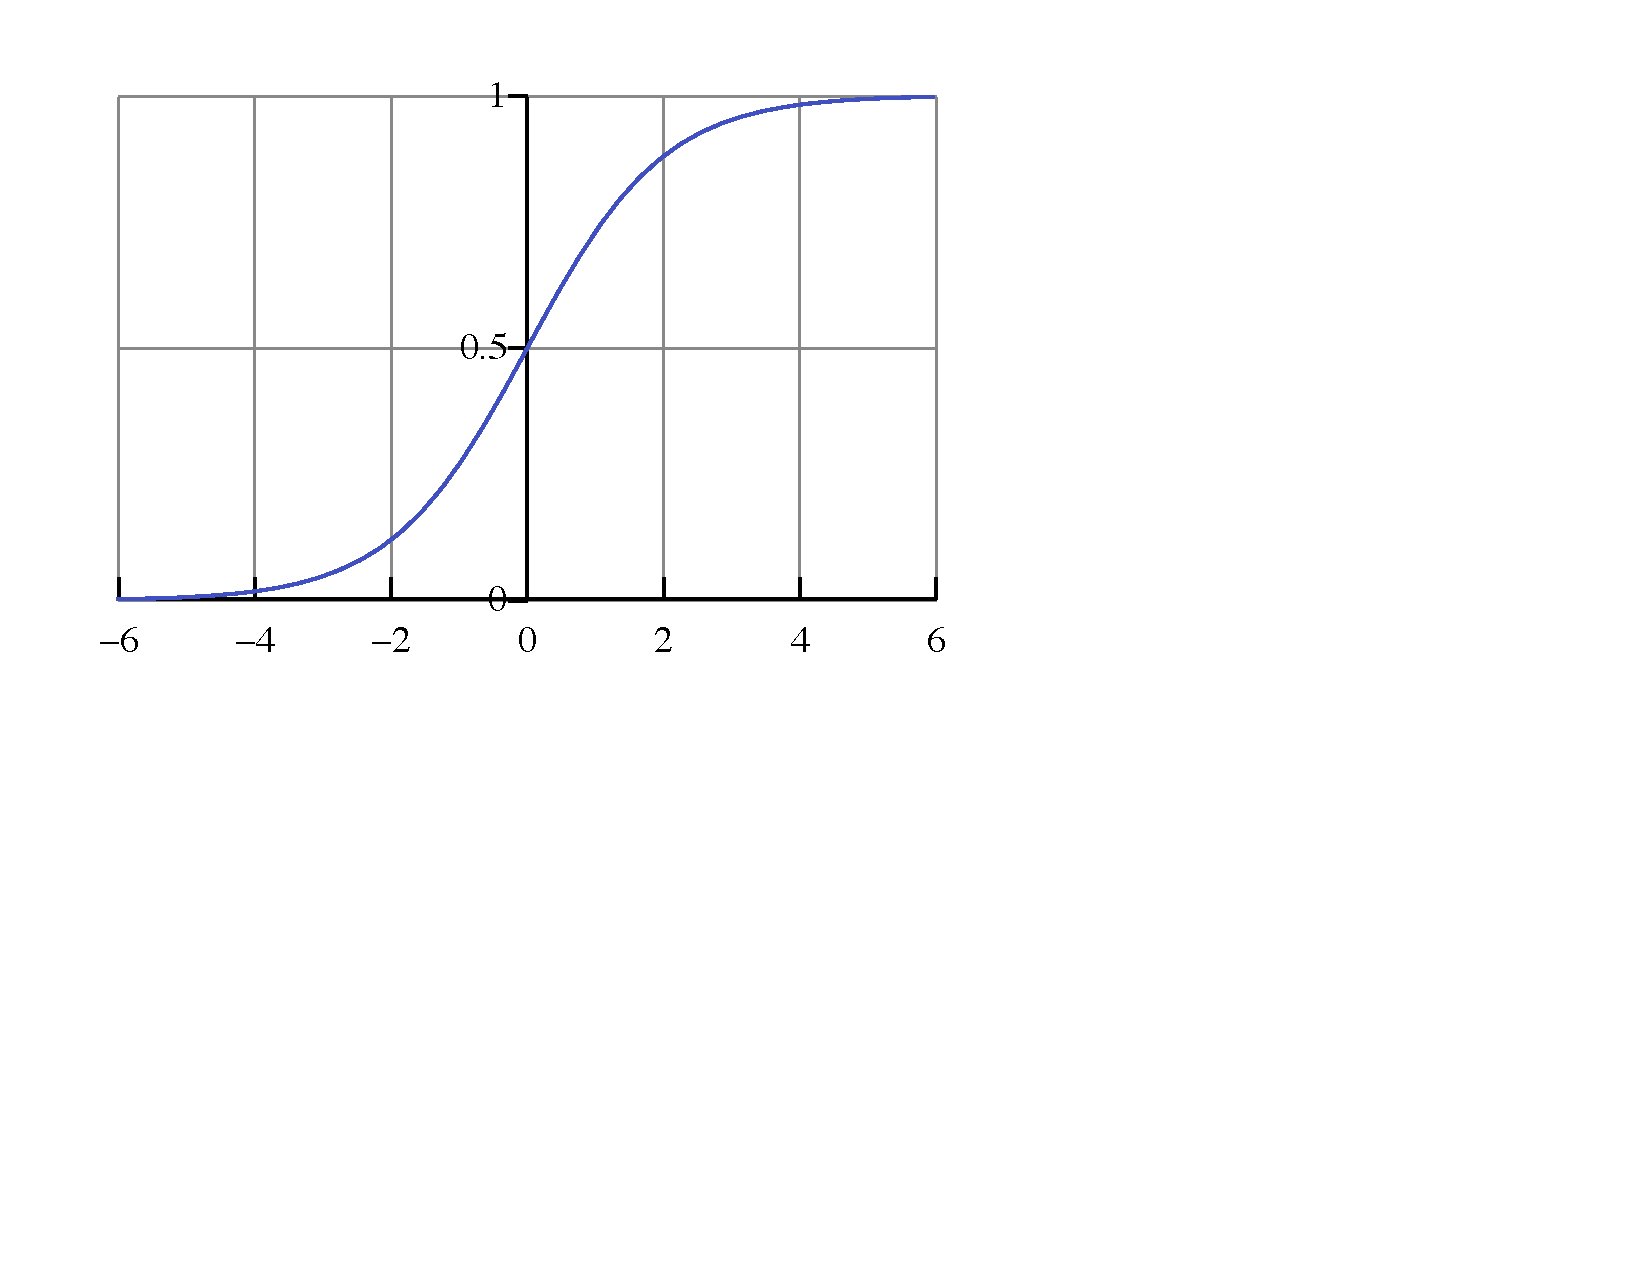
\includegraphics[width=\linewidth]{figures/Logistic-curve}
\caption{fasf}\label{fig:sigmoid}
\end{marginfigure}
\ee

As motivating example, consider what would happen if we were faced with learning the following task.

\href{https://archive.ics.uci.edu/ml/datasets/Occupancy+Detection+}{The dataset} can be found at the UCI Machine Learning repository.  was presented in the paper \href{https://www.sciencedirect.com/science/article/pii/S0378778815304357}{Accurate occupancy detection of an office room from light, temperature, humidity and CO2 measurements using statistical learning models}

\begin{table}
\begin{tabular}{c | c}
2 & 2
\end{tabular}
\end{table}

TODO: state the objective function.

\subsection{Example}
Todo: link to notebook

\section{Gradient Descent}

TODO: Link out to a resource here.

\section{Chain Rule for Gradients}
It turns out that when we are fitting the parameters of our logistic regression model we are going to use the technique of gradient descent in order to compute the optimal weights.  Looking back at Equation~REFTOOBJECTIVE, we see that in order to compute a gradient we will have to compute the gradient of $\mathbf{x}^\top \mlvec{w}$ with respect to $\mlvec{w}$ (which we know how to do from the last assignment).  Additionally, we will have to understand how the application of the sigmoid function and the log function change this gradient.  In this section we'll learn some rules for easily computing gradients in such situations.

In the past assignment you dusted off some old tricks from single variable calculus.  You may have applied the chain rule for derivatives.  The chain rule tells us how to compute the derivative of the composition of two single variable functions $f$ and $g$.  

\begin{align}
h(x)&= g(f(x))&\mbox{h(x) is the composition of $f$ with $g$} \nonumber \\
h'(x) &= g'(f(x))f'(x)&\mbox{this is the chain rule!}
\end{align}

Suppose that instead of the input being a scalar $x$, the input is now a vector, $\mlvec{w}$.  In this case $h$ takes a vector input and returns a scalar, $f$ takes a vector input and returns a scalar, and $g$ takes a scalar input and returns a scalar.

\begin{align}
h(\mlvec{w}) &= g(f(\mlvec{w}))&\mbox{h($\mlvec{w}$) is the composition of $f$ with $g$} \nonumber \\
\nabla_{\mlvec{w}} h(\mlvec{w}) &= g'(f(\mlvec{w})) \nabla_w f(\mlvec{w}) & \mbox{this is the multivariable chain rule}
\end{align}

\begin{exercise}
\bes
\item Compute the gradient of $h(\mlvec{v}) = (\mlvec{c}^\top \mlvec{v})^2$.
\begin{boxedsolution}
We can see that $h(\mlvec{v}) = g(f(\mlvec{v}))$ with $g(x) = x^2$ and $f(\mlvec{v}) = \mlvec{c}^\top \mlvec{v}$ The gradient can now easily be found by applying the chain rule.

\begin{align}
\nabla h(\mlvec{v}) &= 2(\mlvec{c}^\top \mlvec{v}) \mlvec{c}
\end{align}
\end{boxedsolution}
\item This should be punted until the known the derivative of sigmoid function: Compute the gradient of $h(\mlvec{w}) = \frac{1}{1+e^{-\mlvec{w}^\top \mlvec{x_i}}}$ (hint: this is $\sigma(\mlvec{w}^\top \mlvec{x_i})$).
\begin{boxedsolution}
We can see that $h(\mlvec{w}) = g(f(\mlvec{w}))$ with $g(x) = \sigma(x)$ and $f(\mlvec{w}) = \mlvec{w}^\top \mlvec{x_i}$ The gradient can now easily be found by applying the chain rule.

\begin{align}
\nabla h(\mlvec{v}) &= \sigma(\mlvec{w}^\top \mlvec{x_i})(1 - \sigma(\mlvec{w}^\top \mlvec{x_i}) ) \mlvec{x_i}
\end{align}

\end{boxedsolution}
\ees
\end{exercise}

\section{Deriving the Learning Rule for Logistic Regression}

\subsection{Useful Properties of the Sigmoid Function}

The sigmoid function\sidenote{the sigmoid function is a special case of the logistic function.  It is common to see it referred to in be either name} known as a logistic function) turns out to be very useful for modeling the probability that some event occurs.  TODO.

\begin{exercise}
In this exercise you will be working to better understand some of the properties of the logistic function.  Remember, the logistic function, $\sigma$, is defined as:

\begin{align}
\sigma(x) &= \frac{1}{1+e^{-x}} \enspace .
\end{align}

\bes
\item Do some thought exercises on the logistic function.  Limiting cases, etc. TODO.
\item Show that $\sigma(-x) = 1 - \sigma(x)$.
\begin{boxedsolution}
\begin{align}
\sigma(-x) &= \frac{1}{1+e^{x}} \\
&= \frac{e^{-x}}{e^{-x} + 1}~~\mbox{multiply by top and bottom by $e^{-x}$} \\
 \sigma(-x)  - 1&= \ \frac{e^{-x}}{e^{-x} + 1} - \frac{1 + e^{-x}}{1 + e^{-x}} ~~\mbox{subtract $-1$ on both sides} \\
 &= \frac{-1}{1+e^{-x}} \\
 &= -\sigma(x) \\
 \sigma(-x) &= 1 - \sigma(x)
\end{align}
\end{boxedsolution}
\item Show that the derivative of the logistic function $\frac{d}{dx} \sigma(x) = \sigma(x) (1 - \sigma(x))$

\begin{boxedsolution}
Two solutions for the price of 1!

Solution 1:
\begin{align}
\frac{d}{dx} \sigma(x)  &= -e^{-x} \sigma(x)^2 &\mbox{\href{https://www.math.hmc.edu/calculus/tutorials/quotient_rule/}{apply quotient rule}} \\
&= \sigma(x) \left ( \frac{-e^{-x}}{1 + e^{-x}} \right) &\mbox{expand out one of the $\sigma(x)$'s}\\
&= \sigma(x) \left ( \frac{-1}{e^{x} + 1} \right) & \mbox{multiply top and bottom by $e^{x}$}\\
&=  \sigma(x) ( - \sigma(-x)) &\mbox{substitute for $\sigma(-x)$} \\
&=  \sigma(x) ( \sigma(x) - 1) &\mbox{apply $\sigma(-x)=1-\sigma(x)$}
\end{align}

Solution 2:
\begin{align}
\frac{d}{dx} \sigma(x)  &=\frac{-e^{-x}}{(1+e^{-x} )^2} & \mbox{\href{https://www.math.hmc.edu/calculus/tutorials/quotient_rule/}{apply quotient rule}} \\
&= \frac{-e^{-x}}{1+2e^{-x} + e^{-2x}} & \mbox{expand the bottom}\\
&= \frac{-1}{e^{x}+2 + e^{-x}} & \mbox{multiply top and bottom by $e^{x}$}\\
&= \frac{-1}{(1+e^{x})(1+e^{-x})} & \mbox{factor} \\
&= -\sigma(x)\sigma(-x) & \mbox{decompose using definition of $\sigma(x)$}\\
&= -\sigma(x)(1-\sigma(x)) &\mbox{apply $\sigma(-x)=1-\sigma(x)$} \\
&= \sigma(x)(\sigma(x) - 1) & \mbox{distribute the $-1$}
\end{align}

\end{boxedsolution}
%
%\item \textbf{considering making this optional or just deleting} The log odds of an event occurring is defined as 
%\begin{align}
%\ln \left ( \frac{p(\mbox{event occurs})}{p(\mbox{event does not occur})} \right) = \ln \left ( \frac{p(\mbox{event occurs})}{1 - p(\mbox{event does occur})} \right) \enspace .
%\end{align}
%
%If we assume that $p(\mbox{event occurs}) = \sigma(x)$, show that the log odds of the event occurring is equal to $x$.
%
%\begin{boxedsolution}
%\begin{align}
%\ln \left ( \frac{p(\mbox{event occurs})}{p(\mbox{event does not occur})} \right)  &= \ln \left ( \frac{\sigma(x)}{1 - \sigma(x)} \right ) \\
%&= \ln \left ( \frac{\sigma(x)}{\sigma(-x)} \right ) \\
%&= \ln \left ( \frac{1 + e^x}{1+e^{-x}} \right) \\
%&= \ln \left ( e^x \frac{1 + e^x}{e^{x}(1+e^{-x})} \right) \\
%&= x + \ln \left ( \frac{1+e^x}{e^{x} + 1} \right) \\
%&= x
%\end{align}
%\end{boxedsolution}

\ees

\end{exercise}


Todo: this is easier with the identities of the derivative of a logistic function.

\begin{align}
\mathbf{w^\star} &= \argmin_{\mathbf{w}} e(\mathbf{w}) \\
e(\mathbf{w}) &= \sum_{i=1}^n y_i \log \frac{1}{1 + e^{-\mathbf{w}^\top \mathbf{x_i}}} +  (1-y_i) \log \frac{1}{1 + e^{\mathbf{w}^\top \mathbf{x_i}}} \\
&= \argmin_{\mathbf{w}} \sum_{i=1}^n -y_i \log \left ( 1 + e^{-\mathbf{w}^\top \mathbf{x_i}} \right) -  (1-y_i) \log \left ( 1 + e^{\mathbf{w}^\top \mathbf{x_i}} \right) \\
\nabla e(\mathbf{w}) &= \sum_{i=1}^n \frac{y_i \mathbf{x_i}}{1 + e^{-\mathbf{w}^\top \mathbf{x_i}}} - \frac{\left ( 1 - y_i \right) \mathbf{x_i}}{1 + e^{\mathbf{w}^\top \mathbf{x_i}} } \\
&= \sum_{i=1}^n \mathbf{x_i} \left ( \frac{y_i }{1 + e^{-\mathbf{w}^\top \mathbf{x_i}}} - \frac{\left ( 1 - y_i \right) }{1 + e^{\mathbf{w}^\top \mathbf{x_i}} } \right)
\end{align}

\section{Implementation?}
Todo

\end{document}
